% ---------------------------------------------------------
\chapter{Background and Related Work}
\label{b_rel_work}
% ---------------------------------------------------------

This chapter provides fundamental concepts required to follow this thesis. 
In section~\ref{background} we give an introduction about variability models, performance assessment and performance prediction. 
We summarized related work and approaches that analyse performance similar to our approach in section~\ref{rel_work}.

\section{Background}
\label{background}

We give an overview about configurable software systems~(section~\ref{background_conf_sys}) and variability models~(section~\ref{background_variab_models}). 
We define the term performance~(section~\ref{background_perf}) for this thesis, describe how performance of software can be measured, and how to learn models in order to be able to predict performance.

\subsection{Configurable Software Systems}
\label{background_conf_sys}
% Problem Space (Whole space) - Constraints (illegal feature combinations), default settings, optimizations, ... -> Solution Space ()
% variability models of configurable software systems
Today, almost every software system provides different options for configuration. 
Each combination of configuration options results in a \textit{variant} of the program, similar to \acp{SPL}\footnote{``A \ac{SPL} is a set of software-intensive systems that share a common, managed set of features satisfying the specific needs of a particular market segment or mission which are developed from a common set of core assets in a prescribed way.''~(\cite{northrop2010spl})}~(\cite{siegmund2012spl}). 
Each variant comprises a set of activated configuration options, which are referred to as \textit{features}. 
The combination of features describes the user desired characteristics of the program~(\cite{czarnecki2000generative}).
For example, a database management system provides features such as compression, encryption, or the use of a specific indexing strategy.
Requirements that describe what a system can do are called functional properties~\cite{chung1995using}. 
In addition to the functionality properties of software, there are also non-functional properties to be met, such as performance and energy limitations.
In literature, there exist different definitions of non-functional properties as surveyed by~\cite{glinz2007non}. \cite{davis1993software} defined non-functions properties as all required attributes of the system like portability, reliability, efficiency, human engineering, testability, understandability, and modifiability. Whereas \cite{kotonya1998requirements} defined non-functional properties as all requirements which are not directly related to the functionality of the system. Such requirements set restriction to the development process and specify constraints that the software must met.

In this thesis, we use the definition of~\cite{robertson1999mastering} because these definition is general and has been widely used by others:~\cite{nuseibeh2000requirements,jackson2001problem,cohn2004user,siegmund2012spl}. ``A property, or quality, that the product must have, such as an appearance, or a speed or an accuracy property''.

\subsection{Variability Models}
\label{background_variab_models}

An important requirement when developing and maintaining configurable-software systems is to model the variability in a comprehensible way. 
\textit{Feature models} define a common way to describe all valid configurations of software systems~\cite{kang1990feature,czarnecki2000generative, apel2016feature}. 
They have been introduced by~\cite{kang1990feature} and are usually realized with two different representations: textual notations and graphical representations. 
Feature models in textual from (e.g., SXFM introduced by~\cite{Mendonca2009SSP} and Velvet introduced by~\cite{rosenmuller2011multi}) have been developed to construct and maintain models of systems with a huge amount of features which might be presented poorly with a graphical tool. 
Whereas feature models with a graphical representation (also called feature diagrams~\cite{kang1990feature}) provide the possibility to create and manipulate feature models through a graphical user interface. 
Furthermore, feature diagrams are widely used in scientific literature to present analyzed systems. 


Feature diagrams build up a tree-structured graph, as can be seen in the example diagram shown in Figure~\ref{background_variab_models_feature_diagram_example}. 
With this example diagram, we will describe the elements of feature diagrams. 
The root node of the tree \textsf{Database\_Engine} represents the whole database model. 
All nodes in this tree represent either \textit{abstract} or \textit{concrete} features. 
Abstract features such as \textsf{Compression} and \textsf{OS} are used to structure the feature model, whereas concrete features represent functionality that maps to implementation units. 
Two nodes of the database engine are modelled as \textit{mandatory}. 
These nodes have to be selected in each valid configuration because they might implement some basic functionality which has to be always available. 
Optional features such as \textsf{Indexing} or \textsf{Compression} can be selected to create a valid variant with additional functionality.
For example, all databases need to have an operating system specified and can optionally use compression algorithms. 
There are two more elements available in feature diagrams: \textit{or}- and \textit{alternative} groups. 
The \textit{alternative} group represents the logical XOR, hence only one child must be selected at a time, whereas the \textit{or} group enables the selection of one or more children. 
If \textsf{Encryption} is selected in this example, either \textsf{AES} or \textsf{RSA} or both must also be selected. 
In case of the mandatory abstract feature \textsf{OS} which itself only groups available operation systems, one has to select either \textsf{Unix} or \textsf{Windows}. 
The structure of the tree, including the parent-child relationship and the different elements, defines a set of constraints for selecting valid configurations.
Additionally, there are also \textit{cross-tree constraints} which represent logical expressions over the set of features. 
They enable the modelling of arbitrary formulas amongst the features in feature models.
For example, if users want to have zip-compression enabled, they also have to stick to Windows. 
Such constraints restrict the amount of valid configurations. 
In total, our example has 64 valid configurations. 
If \textsf{Windows} is initially selected there are 24 valid configurations and if \textsf{Unix} is selected we can derive 40 valid configurations.
The textual representation of the feature model is available in the appendix~\ref{app_feature_diagrams}.

\begin{figure}
  \centering
  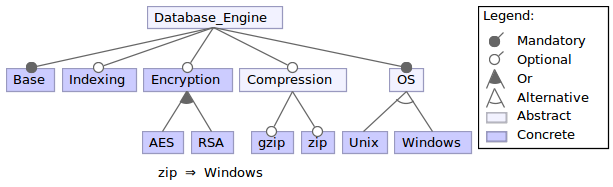
\includegraphics[width=0.8\textwidth]{images/example_database}
  \caption{Example database model (extended form section~\ref{background_conf_sys}).}
  \label{background_variab_models_feature_diagram_example}
\end{figure}

\subsection{Performance Assessment}
\label{background_perf}

Next, we define performance for this thesis and show how to assess performance to learn models from measured configurations. 
Afterwards, we present different approaches of how these models can predict performance.

\subsubsection{Performance in Software Engineering}
\label{perf_general}

Performance is an important quality of software systems. 
As described in the introduction, definitions of performance differ depending on the perspective. 
The most used way is to explain performance of software systems as a non-functional property (\cite{Molyneaux:2009:AAP:1550832,liggesmeyer2002software}). 
Here, performance is a mean for describing how a system provides its functionality. 
To decide if a system performs well, non-functional properties are compared to so called \acp{NFR}. 
They constitute a set of requirements which the software should fulfil. 
\acp{NFR} should be defined before the software is tested. 
Each type of a software system has different metrics which can be analysed. 
For example, a Web server can be analyzed through the following metrics:

\begin{description}[style=multiline,leftmargin=10em]
	\item [Hit Rate] is the total number of requests arriving at a server in a defined time frame.
	\item [Latency] describes the time that has passed from the start of a request message until the response message starts being received.
	\item [Response Time] describes the time that has passed from the start of a request message until the whole response message is received.
	\item [Availability] describes the time that the software is available to the user.
\end{description}

With client-server applications, communication takes place through networks, whereas with offline applications, the focus during the analysis of performance metrics lies on the intrinsic properties.
Offline applications usually run on a single device and do not need to communicate directly with other systems. 
The following are some performance metrics of offline applications:

\begin{description}[style=multiline,leftmargin=10em]
	\item [Resource Utilization] describes the fraction to which a system uses its resources\footnote{A resource is a system element that offers some service to other system elements that require them. Resources can be categorized into hardware components (CPU, bus, storage), logical elements (buffers, locks, semaphores) and processing resources (processes, threads)~\cite{woodside2007future}.}.
	\item [Response Time] describes the time that is needed to complete an operation.
	\item [Throughput] is the amount of work done in a defined time.
	\item [Availability] describes the time that the software is available to the user.
	\item [Scalability] describes the ability to grow and perform an increasing amount of work. 
\end{description}

For this thesis, we will focus on offline systems because we do not want to cope with the measurement inaccuracy which might accompany with the hardware and software of networks resources. 
Furthermore, we want to define performance as the amount of work done per unit of time like~\cite{tsirogiannis2010analyzing}. 
So, we define performance as:
\begin{equation}
	\label{def:perf1}
	\mbox{Performance}=\frac{\mbox{Work Done}}{\mbox{Execution Time}}
\end{equation}

Because we want to analyze performance of configurable software systems, we execute different variants of each system using the same inputs (benchmarks\footnote{Benchmarking is the process of running a software system with standardized workloads to be able to compare the results and assess their relative performance.}) for all configurations. 
Thereby, we are able to compare the different variants and since the \textsf{Work Done} is constant, we are able to simplify our formula like~\cite{siegmund2015performance}:

\begin{equation}
	\label{def:perf2}
	\mbox{Performance}=\frac{\mbox{1}}{\mbox{Execution Time}}
\end{equation}

%Because we want to analyze performance of software by executing benchmarks, the work done is always the same. So for this thesis we can define performance like~\cite{siegmund2015performance}:

To identify performance hot-spots, we also measure the run time of each method that is executed.
We are interested in the time spent in each method (net-time).
We explain the concrete approach we follow in this thesis in section~\ref{perf_measure}. 


\subsubsection{\ac{SPE}}

After defining performance in general, we outline the process of analyzing performance of software systems.
The process of analyzing performance of software systems is defined as follows:
\begin{quote}
``\ac{SPE} represents the entire collection of software engineering activities and related analyses used throughout the software development cycle, which are directed to meeting performance requirements.''~(\cite{woodside2007future}).
\end{quote}
There are two general approaches in the literature (\cite{woodside2007future}): \textit{measurement-based} and \textit{model-based} performance assessment. 
The model-based approach is applied early in the development cycle. 
It tries to create performance models to adjust design and architecture as early as possible. 
The measurement-based approach is applied late in the development cycle, because it will run tests and diagnosis to tune the software.
The whole process of \ac{SPE} activities can be structured into six parts (\cite{woodside2007future}). 
The first identifies the \ac{NFR} which should be analysed.
Defining and analyzing the requirements is the second step. 
This includes specifying the environment in which the software runs. 
For the sake of reproducibility, the environment should be defined carefully.  
To select specific tasks, there are many different benchmarks available (\href{https://bapco.com/}{BAPCo}, \href{https://www.eembc.org/}{EEMBC}, \href{http://www.spec.org/}{SPEC}). 
These and other benchmarks provide the possibility to compare one software variant to another with a set of standardized tests and workloads. 
Another possibility is to use benchmarks which are provided by the software vendor itself (a concrete example is provided in section~\ref{case_studies}). 
This may enable analysis of the whole functionality of a the software system.
The third activity is to design models that can predict performance from detailed design, architecture, and usage scenarios. 
These models describe how systems use resources and how resource contention affects operation. 
These models are able to predict system properties before they are implemented to gather knowledge as early as possible in the software development life cycle.
The next \ac{SPE} activity is performance testing. 
Tests can cover only parts or the entire software, depending on the selected benchmarks. 
Here, we obtain actual values for the performance metrics we selected.
From the gathered data, we can learn models to predict the effect of changes to the system, which is the fifth step of \ac{SPE}. 
A lot of effort has been spent in the last years to understand and improve performance. 
Section~\ref{rel_perf_pred} summarizes more recent measurement-based performance prediction approaches which emphasize variability.
The last step of \ac{SPE} is to analyze the whole system.
Here, the final deployed system is analyzed regarding to the defined performance goals.

This thesis identifies concerns, conducts performance tests and learns models for performance prediction of configurable software systems. 
Because we follow the \textit{measurement-based} approach, we also evaluate the impact of the measurement environment. 


\section{Related Work}
\label{rel_work}

This section cope the topics performance prediction and performance analysis of Java programs. The first part deals with different approaches on learning the influence of feature selection on performance and presents different sampling strategies. The second part reviews existing performance analysis tools.

% Performance in software systems
\subsection{Performance Prediction}
\label{rel_perf_pred}

The task of learning and predicting performance is subject of research for several years. Since then, several measurement-based performance prediction models were developed. In general, they all work the same way. They sample a subset of configurations because measuring performance of each configuration is not practicable if the configuration space is too big. They split the available measurements into two sets (learning set and test set). For learning a model, they use the learning set and to be able to assess the accuracy of the model they compare the test set with the prediction of the model. In the following, we describe the differences of some models.

One task of \acp{SPL} is to express the large number of possible products. \cite{thum2012family} presented the approach, called family-based verification, in which the whole \ac{SPL} is encoded in a single \textit{meta-product} which simulates the behaviour of all individual products of the product line. The idea is to verify only the generated meta-product. It contains the implementation and specification of every feature. So, it is able to simulate each product. They verify the meta-product (family-based) instead of verifying all products separately (product-based). Because of the generation of the meta-product, they do not have different products from a product line, but a single system, so they are able to use the single-system theorem prover KeY for verification. They adapted the product simulator introduced by~\cite{apel2011detection} to translate the Java-based product line into the meta-product. In comparison to the product-based approach, the authors were able to save more than 85\% of the verification effort.

\cite{guo2013variability} presented a variability-aware approach to performance prediction. The authors want to use few samples (linear in the number of features) to show that this is enough to learn a model that can accurately predict performance of all configurations. They make use of \acp{CART} to recursively partition the configuration space into smaller segments. The mean performance value of the samples of each segment is used as local prediction model. The prediction error at each segment is calculated through the sum of squared error loss. Each split is chosen according to the feature that reduces the entropy of the resulting subsets most. The configuration space will be further subdivided until each leaf of the tree locally describes the configuration best. They introduce two parameter which control the recursive partitioning process to prevent underfitting and overfitting: minibucket is the minimum sample size for any leaf of the tree; and minisplit is the minimum sample size of each segment before it is considered for further partitioning. After that, the algorithm adds iteratively new measured samples and rebuilds the performance model.

\cite{siegmund2012spl} presented an holistic approach, \textit{SPLConqueror}, to optimize learning the influences of features on \ac{NFP}. They automate the process of learning the influence of features and their interactions on performance, including sampling, measurement, and creation of performance influence models. They differentiate between feature-wise (i.e., measure an implementation module of a feature in isolation and independent of the remaining software system) and variant-wise assessment (i.e., assessing a property that emerges only when running a valid variant). They also introduce two sampling strategies to analyze the influence of individual features as well as the influence of feature interactions. With \textit{feature-wise} sampling the influence of individual features \textit{f} to \acp{NFP} is analyzed by sampling two variants of each feature. The first variant selects feature \textit{f} and the other variant deselects feature \textit{f} while in both variants the number of additionally selected features is minimized. So the difference between these two variants present the impact of feature \textit{f} on the \ac{NFP}. The other sampling strategy (\textit{pair-wise} sampling) works similar but uses each combination of two features.

\cite{siegmund2012predicting} have further developed the idea of automated detection of feature-interactions. Feature interactions occur when a particular feature combinations have an unexpected influence on performance. They wanted to detect performance-relevant feature interactions to reduce the amount of samples needed to create a performance-influence model. At the start, they identified the set of features that interact with other features by applying a heuristic: If the distance between $\Delta a_{max}$ and $\Delta a_{min}$ is within a threshold feature $a$ does not interact with other features. The deltas of $a$ are the two that are most likely to differ because $\Delta a_{min}$ is the delta of the minimum number of features selected, whereas with $\Delta a_{max}$ most features are selected. The set of features that are likely to interact with each other is created through applying this heuristic to each feature. Then three additional heuristics are applied to identify feature combinations that cause interactions. First, they investigate candidates for pair-wise interaction. In the second step they used these candidates to identify higher-order interactions (i.e., interactions among three features). Finally, hot-spot features are derived from the set of pair-wise and higher-order interactions. They interact with many other features, and are therefore interesting for optimization.

A further development of the idea of how to build performance-influence models was introduced by \cite{siegmund2015performance}. They extend the tool \textit{SPLConqueror} to create human understandable models that describe the performance behavior of features, interactions, and variants. The distinguishing aspect of this work is that they also support numerical features. Therefore, they applied different binary (e.g., pair-wise, option-wise, negative option-wise) and numerical (e.g., Placket-Burman Design) sampling strategies\footnote{We will give an overview of sampling strategies in section \ref{perf_measure_sampling}.} and combined them. The learning procedures consists of a combination of multi-variable regression and feature subset selection as dimensionality-reduction technique. Linear regression tries to fit a line through measurement points by adjusting regression coefficients so that the global error is minimal. The proposed approach incrementally adds new regression terms to the formula in each round until a certain accuracy is reached or improvement in accuracy becomes marginal.

\cite{sarkar2015cost} proposed another approach to further reduce the number of samples needed to learn an accurate performance model. The authors want to dynamically determine an ideal sample size dynamically, that yields a good prediction accuracy with low measurement effort. They investigate two sampling strategies (projective sampling and progressive sampling) which both are used in data mining to reduce the size of data needed. After sampling, they use CART to build the prediction model. A typically evaluation criteria is prediction accuracy, but \cite{sarkar2015cost} use an accumulated cost function consisting of (weighted) prediction error and costs for creation of test and training sets. With their approach, they are able to reduce the number of elements needed for an initial sample. 

All aforementioned approaches rely on improving certain aspects of configurable software systems (or \ac{SPL}) modelling. They provide new strategies for sampling or present tools for learning performance models. However, they all utilize black-box approaches that analyzes the examined software systems as a whole. We, however, want to create and analyze performance model on method-level, which was not addressed so far.

\subsection{Performance Analysis of Java Programs}
\label{rel_perf_java}

To the best of our knowledge there exist no approach that models and predicts performance on method level of a configurable software system (written in Java). Nevertheless, there is related work in monitoring and assessing performance of monolithic Java applications.

\cite{vanHoorn2012kieker} present a framework, \textit{Kieker}, for monitoring and analyzing the runtime behaviour of software systems. They target monitoring the runtime behaviour of concurrent and distributed applications. Their tool is able to collect time and tracing information as well as sampling system-level measurements (CPE utilization and memory usage). \textit{Kieker} also provides logging and streaming mechanisms to save the data for later analysis or to visualize incoming records directly. Furthermore, it achieves an average monitoring overhead of about 10\% and is recommended by the SPEC Research Group.

Another tool which adapts Java bytecode is \textit{SPASS-meter} introduced by \cite{eichelber12spassmeter}. Similar to \textit{Kieker}, it instruments the bytecode to profile \acp{NFP} such as throughput or response time. It is also capable of logging CPU-usage of the \ac{JVM} or memory usage. The monitoring overhead which accompanies with instrumentation is comparable to that of \textit{Kieker}. Also memory overhead caused by logging the measurements does not differ substantially. 

The list of performance monitoring and analysis frameworks is not exhaustive. Here, we focus on open-source tools that approaches recently to motivate our decision on providing additional support in the field of variability-aware performance analysis of software systems. \textit{Kieker} as well as \textit{SPASS-meter}, do not support handling configurable software systems in combination with variability modelling. Nevertheless, they can represent a powerful tool to assess performance of single variants at method level from which we can derive performance models.